\documentclass[journal,10.75pt,twocolumn]{IEEEtran}
\usepackage{graphicx, float}
\graphicspath{{./figs/}}{}
\usepackage{amsmath,amssymb,amsfonts,amsthm}
\newcommand{\myvec}[1]{\ensuremath{\begin{pmatrix}#1\end{pmatrix}}}
\usepackage{listings}
\usepackage{watermark}
\usepackage{titlesec}
\let\vec\mathbf
\lstset{
frame=single, 
breaklines=true,
columns=fullflexible
}

\title{\mytitle}
\title{
Matrix Assignment - Circle
}
\author{Pratheek Darla}
\date{October 2022}

\begin{document}
\maketitle
\tableofcontents
\bigskip


\section{\textbf{Problem}}
For the circle $x^2+y^2= r^2$ , find the value of r for which the
area enclosed by the tangents drawn from the point P (6, 8)
to the circle and the chord of contact is maximum.\\


\section{\textbf{Solution}}
The equation of a circle is given as,   \\

\begin{equation}
{\vec{x^{\top}V x} + 2\vec{u^{\top}x}} + f=0 \label{eq-1}
\end{equation}

The circle given in the question can be written in the above form as follows
\\

$\myvec{x & y}\myvec{1&0\\ 0&1}\myvec{x\\y} + 2\myvec{0&0}\myvec{x\\y} + f = 0$\\
\\
where,
\\
\begin{equation}
\vec{V}=\myvec{1&0\\ 0&1} , \vec{u^{\top}}=\myvec{0&0} , f=-r^2 \label{eq-2}
\end{equation}


The points of contact of the two tangents drawn from the given external point P to the circle can be found from the following equation
\\
\begin{equation}
\boxed{\vec{q}_i = \vec{V^{-1}}(k_i\vec{n_i-u})}  ....(i = 1,2) \label{eq-3}
\end{equation}

here,
\\
\begin{equation}
k_i = \pm\sqrt{\frac{f_0} {\vec{n^T} \vec{V^{-1}} \vec{n}}} \label{eq-4}
\end{equation}

\vspace{0.2cm}

\begin{equation}
f_0 = \vec{{\vec{u^T} \vec{V^{-1}} \vec{u}}}-f \label{eq-5}
\end{equation}

\vspace{0.2cm}

\begin{equation}
n_1 = \vec{P}\myvec{\sqrt{|\lambda_1|} \\ \sqrt{|\lambda_2|}} \label{eq-6}
\end{equation}

\vspace{0.2cm}

\begin{equation}
n_2 = \vec{P}\myvec{\sqrt{|\lambda_1|} \\ -\sqrt{|\lambda_2|}} \label{eq-7}
\end{equation}

\vspace{0.2cm}

\begin{align}
\vec{P} = (\vec{Vh+u})(\vec{Vh+u})^T-\vec{V(h^TVh+2u^Th}+f) \label{eq-8}
\end{align}
\\
On solving the above equations by substituting the values in (\ref{eq-2}), we get two point of contacts of tangents to the circle in terms of 'r',

\begin{equation}
\vec{q_1} = -r/10 \begin{pmatrix}
{-0.8 \sqrt{100 - r^2} - 0.6r} \\
{0.6 \sqrt{100 - r^2}} -0.8r 
\end{pmatrix}  \label{eq-9}
\end{equation}

\begin{equation}
\vec{q_2} = r/10 \begin{pmatrix}
{-0.8 \sqrt{100 - r^2} + 0.6r} \\
{0.6 \sqrt{100 - r^2}} + 0.8r 
\end{pmatrix}  \label{eq-10}
\end{equation}

\vspace{0.2cm}

Let these two points be $\vec{A}$ and $\vec{B}$. Then the area of the triangle with vertices $\vec{P}, \vec{A}, \vec{B}$ is given by
\\

\begin{equation}
	\frac{1}{2} (\left ||(\vec{P-A})\times(\vec{P-B})|| \right) \label{eq-11}
\end{equation}
\vspace{0.2cm}

where, $\vec{P} = \myvec{6 \\ 8}$
\\

By substituting the values in (\ref{eq-11}) and solving, we get the area of the triangle in terms of 'r' as follows,
\\
\begin{equation}
f(r) = \frac{r}{100} (100 - r^2)^{\frac{3}{2}}  \label{eq-12}
\end{equation}

\subsection{\textbf{Gradient ascent}}
Using gradient ascent method we can find the value of 'r' for which the area of the triangle with vertices $\vec{P},\vec{A},\vec{B}$ is maximum,
\\

$\implies r_{n+1} = r_n + \alpha \nabla f(r_n) $\\
\begin{equation*}
    \implies r_{n+1}=r_n+\alpha \nabla(\frac{(100-r^2)^{\frac{3}{2}}-3r^2(100-r^2)^{\frac{1}{2}}}{100})
\end{equation*}

\vspace{0.2cm}

Taking $r_0=0.5,\alpha=0.0001$ and precision = 0.000000001, values obtained using python are:
    \begin{align}
        \boxed{\text{Maxima} = 32.47595264190203}\\
        \boxed{\text{Maxima Point} = 4.9999971149068765}
    \end{align}

\vspace{0.2cm}

The maxima point can be rounded to 5.0.
\\
So, the value of 'r' for which the area enclosed by the tangents drawn from the point P (6, 8) to the circle and the chord of contact is maximum is 5.

\begin{figure}[h]
    \centering
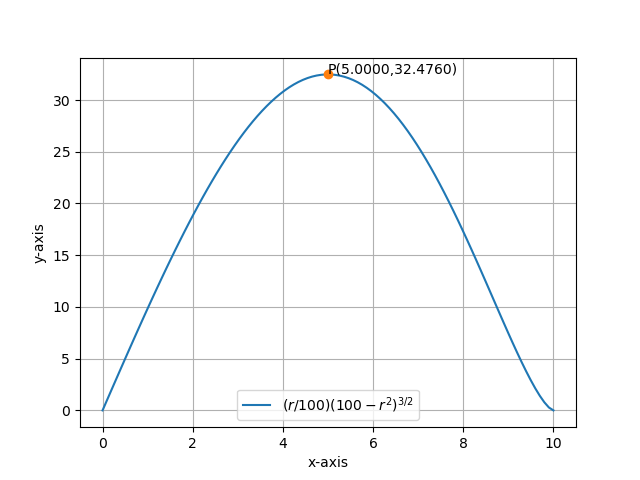
\includegraphics[width=\columnwidth]{figs/fig-opt.png}
    \label{fig:my_label}
\end{figure}

\section{\textbf{Figure}}
\begin{figure}[h]
    \centering
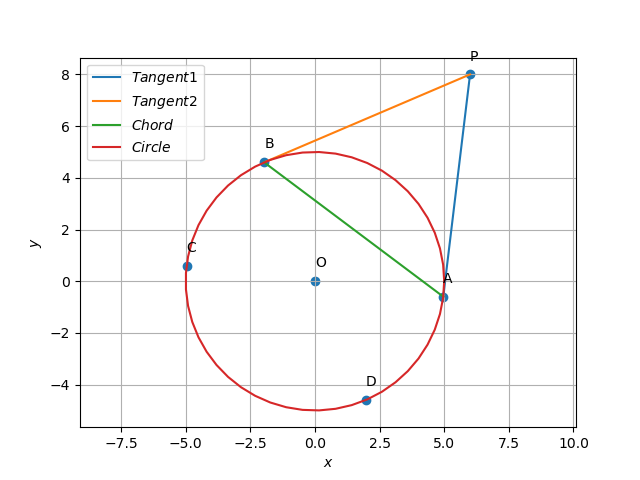
\includegraphics[width=\columnwidth]{figs/fig-circle1.png}
    \label{fig:my_label}
\end{figure}

\section{\textbf{Code Link}}

\begin{lstlisting}
https://github.com/PratheekDarla/FWC-IITH/blob/main/Matrix/Circle/circle-assignment.py
\end{lstlisting}
Execute the code by using the command\\
\textbf{python3 circle-assignment.py}

\end{document}
